\chapter{腐蚀与防护}\label{ch:b2:corrosion}

在一块干净的钢片上滴一滴盐水，一天后金属
液滴中心出现麻点，而铁锈则在靠近
边缘处形成一圈，那里正是空气中的氧溶解之处。铁在
氧最少处溶解，而氧在氧最多处被还原：这一液滴
就是一个无人组装的电池，经由金属本身短路。
本章借助电流–电势曲线讨论腐蚀，解释为何
划伤的镀锌板不生锈，而划伤的马口铁罐却会生锈，
并设计一条埋地管道的防护方案。

\begin{recall}
本科一年级分册：金属的 E–pH 图及其免蚀区，
腐蚀与钝化（“镀层能否起保护作用，是动力学问题”）。
\Cref{ch:b2:current-potential-curves}：电流–电势曲线，极限
电流。\Cref{ch:b2:batteries-electrolysis}：混合电势。第 1 册
中的腐蚀、铁锈与镀锌。
\end{recall}

\begin{omfigure}
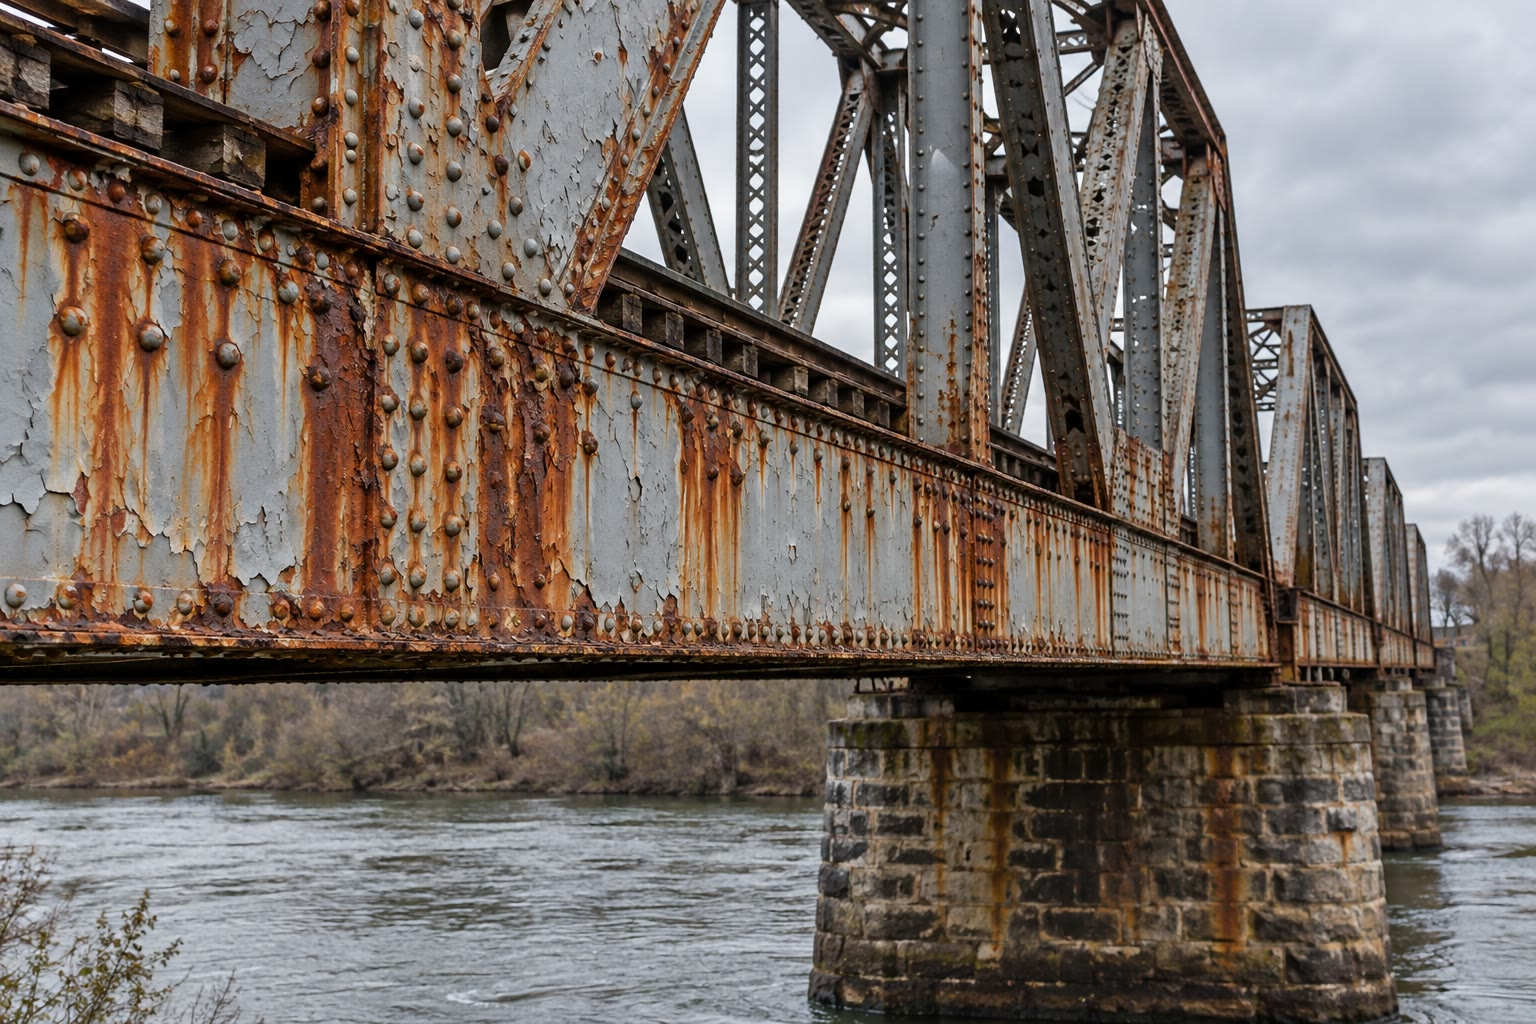
\includegraphics[width=0.62\linewidth]{images/book3/ai/b2-12-rusty-bridge.jpg}

{\small 一座老式铆接铁路桥。锈迹自铆钉
与接缝处向下流淌，那里水和氧停留最久，油漆
最先失效。}
\end{omfigure}

\section{作为短路电池的湿腐蚀}

在溶有氧气的水中，铁被氧化，\ce{Fe -> Fe^2+ + 2e-}，
电子在同一金属片上被
氧气还原所消耗，\ce{O2 + 2H2O + 4e- -> 4OH-}（在酸性介质中，还可通过 \ce{2H+ + 2e- -> H2} 发生还原）。
亚铁离子与氢氧根离子在水中相遇，并经空气进一步氧化，
其沉淀转化为铁锈，即水合氧化铁（III）。

\begin{definition}[均匀腐蚀]\label{def:b2:corrosion:uniform}
\emph{均匀腐蚀}\index{均匀腐蚀}是指一种金属的腐蚀，
其氧化及氧化剂的还原发生在表面
均匀分布的位点上。称\emph{腐蚀电势}\index{腐蚀电势}为
金属此时所取的混合电势，并称
\emph{腐蚀电流}\index{腐蚀电流}为
该电势下金属氧化的阳极电流。
\end{definition}

\begin{omfigure}
\begin{tikzpicture}
\begin{axis}[omie, width=0.82\linewidth, height=5.6cm, xmin=-1.1, xmax=0.5,
  ymin=-1.6, ymax=1.6, xlabel={$E$}, ylabel={$i$}, clip=true, clip mode=individual,
  axis y line=left]
\addplot[omanodic] table[x=E, y=i] {figdata/out/bachelor-2-ie-curves-i-Fe.dat};
\addplot[omcathodic] table[x=E, y=i] {figdata/out/bachelor-2-ie-curves-i-O2.dat};
\addplot[omcathodic, densely dashed] table[x=E, y=i, y expr=-\thisrow{i}] {figdata/out/bachelor-2-ie-curves-i-O2.dat};
\draw[densely dotted] (axis cs:-0.394,-1.0) -- (axis cs:-0.394,1.0);
\fill (axis cs:-0.394,1.0) circle (1.4pt);
\node[font=\scriptsize, anchor=south east] at (axis cs:-0.40,1.02) {$i_{\text{corr}}$};
\node[font=\scriptsize, anchor=north west] at (axis cs:-0.39,-0.03) {$E_{\text{corr}}$};
\node[font=\scriptsize, omThm, anchor=west] at (axis cs:-0.35,1.4) {\ce{Fe} $\to$ \ce{Fe^2+}};
\node[font=\scriptsize, omDef, anchor=north west] at (axis cs:-0.75,-1.05) {\ce{O2} $\to$ \ce{OH-}，扩散平台};
\end{axis}
\end{tikzpicture}

{\small 铁在充气中性水中的埃文斯图（模型曲线）。
氧气的阴极曲线还以虚线向上镜像画出：
腐蚀电势为其与铁阳极曲线的交点。此处氧气的
还原已达扩散平台，故腐蚀电流等于氧的
极限电流：搅拌或充气会使水中的铁
腐蚀更快。}
\end{omfigure}

\begin{proposition}[腐蚀速率]\label{prop:b2:corrosion:rate}
一种摩尔质量为 $M$、密度为 $\rho$ 的金属，每个原子转移
$n$ 个电子而被氧化，在腐蚀电流密度 $j_{\text{corr}}$（单位面积上的电流）下，
则每单位面积、每单位时间损失的质量为 $j_{\text{corr}}M/(nF)$，即
厚度减少的速率为
\[
  \frac{de}{dt} = \frac{j_{\text{corr}}\,M}{nF\rho} .
\]
\end{proposition}

\begin{proof}
由\cref{prop:b2:current-potential-curves:current-rate}可知，阳极电流
密度 $j_{\text{corr}}$ 可使每单位面积、每单位时间氧化 $j_{\text{corr}}/(nF)$ 摩尔的金属；
乘以 $M$ 得质量，除以 $\rho$ 得厚度。
\end{proof}

\begin{example}[铁在 \qty{10}{\micro A/cm^2} 下]\label{ex:b2:corrosion:rate}
取 $j = \qty{0.10}{A/m^2}$，$M = \qty{55.845}{g/mol}$，$n = 2$，$\rho =
\qty{7.87}{g/cm^3}$：$de/dt = 0.10 \times 55.845/(2 \times 96\,485 \times 7.87
\times 10^6) = \qty{3.7e-12}{m/s}$，即每年 \qty{0.12}{mm}。
% ledger: aw:Fe, rho:Fe, const:F
\end{example}

\section{差异腐蚀}

\begin{definition}[差异腐蚀]\label{def:b2:corrosion:differential}
\emph{差异腐蚀}\index{差异腐蚀}是指阳极与阴极位点彼此分开的
腐蚀，金属优先在阳极位点处被氧化。
两种不同金属电接触且共处同一电解质时，称为\emph{电偶
腐蚀}\index{电偶腐蚀}；
一种金属暴露于含氧量不同的水中时，
称为\emph{差异
充气}\index{差异充气}。
\end{definition}

\begin{proposition}[两种金属接触]\label{prop:b2:corrosion:galvanic}
当两种电接触的金属浸入同一充气水中时，它们
取得同一个混合电势。腐蚀电势较低的金属
成为阳极，腐蚀速度比单独存在时更快；另一金属成为阴极，
氧气在其上被还原，因而受到保护。
\end{proposition}

\begin{proof}
两金属以电阻可忽略的导线相连，二者处于
同一电势，该电势下全部阳极电流之和
等于全部阴极电流之和的负值。较活泼金属的阳极曲线先升高；
在共同电势下，它几乎承担全部阳极电流，而
氧在全部润湿表面上被还原，包括较惰性的金属，
其自身的阳极电流在此处可忽略不计。
\end{proof}

\begin{omfigure}
\begin{tikzpicture}
\begin{axis}[omie, width=0.82\linewidth, height=5.6cm, xmin=-1.1, xmax=0.5,
  ymin=-2.4, ymax=2.4, xlabel={$E$}, ylabel={$i$}, clip=true, clip mode=individual,
  axis y line=left]
\addplot[omanodic] table[x=E, y=i] {figdata/out/bachelor-2-ie-curves-i-Fe.dat};
\addplot[omanodic, densely dashed] table[x=E, y=i] {figdata/out/bachelor-2-ie-curves-j-Zn.dat};
\addplot[omcathodic] table[x=E, y=i] {figdata/out/bachelor-2-ie-curves-i-O2.dat};
\addplot[omcathodic, densely dashed] table[x=E, y=i] {figdata/out/bachelor-2-ie-curves-j-O2Cu.dat};
\fill (axis cs:-0.394,1.0) circle (1.4pt);
\fill (axis cs:-0.794,1.0) circle (1.4pt);
\fill (axis cs:-0.366,2.0) circle (1.4pt);
\draw[densely dotted] (axis cs:-1.1,1.0) -- (axis cs:-0.394,1.0);
\draw[densely dotted] (axis cs:-1.1,2.0) -- (axis cs:-0.366,2.0);
\node[font=\scriptsize, anchor=south west] at (axis cs:-0.38,0.95) {单独的铁};
\node[font=\scriptsize, anchor=west] at (axis cs:-0.35,2.0) {铁 + 铜};
\node[font=\scriptsize, anchor=south east] at (axis cs:-0.80,1.05) {铁 + 锌};
\node[font=\scriptsize, omThm, anchor=north west] at (axis cs:-0.98,0.75) {锌};
\node[font=\scriptsize, omThm, anchor=north west] at (axis cs:-0.55,0.75) {铁};
\node[font=\scriptsize, omDef, anchor=north east] at (axis cs:0.45,-2.05) {\ce{O2} 在铁 + 铜上};
\node[font=\scriptsize, omDef, anchor=north east] at (axis cs:0.45,-1.05) {\ce{O2} 在铁上};
\end{axis}
\end{tikzpicture}

{\small 铁与其他金属耦合（模型曲线）。与锌耦合时，
共同电势降至锌承担阳极电流的水平，铁受保护，
锌发生腐蚀。与铜耦合时，氧还原的阴极面积加倍，
故铁的腐蚀电流也加倍。}
\end{omfigure}

\begin{proposition}[差异充气]\label{prop:b2:corrosion:aeration}
金属暴露于含氧量不同的水中时，充气较差的
区域为阳极并发生腐蚀，充气较好的区域为阴极。
\end{proposition}

\begin{proof}
氧含量较高处，\ce{O2}/\ce{OH-} 电对具有较高的
能斯特电势，且极限电流较大，阴极曲线位置更高，
并延伸得更远。金属为单一导体，只能处于一个电势；
充气较好区域可提供的大阴极电流须由阳极电流平衡，
该阳极电流流向金属易被氧化、受氧还原竞争较少的地方，
即充气较差的区域。氧化
集中发生于此。
\end{proof}

\begin{omfigure}
\begin{tikzpicture}[font=\small, >={Stealth}]
  \fill[black!20] (-4.2,-0.7) rectangle (4.2,0);
  \node[font=\scriptsize] at (3.7,-0.35) {钢};
  \fill[omDef!15] (-3.4,0) .. controls (-2.9,2.2) and (2.9,2.2) .. (3.4,0) -- cycle;
  \draw[thick, omDef] (-3.4,0) .. controls (-2.9,2.2) and (2.9,2.2) .. (3.4,0);
  \fill[omProp!80] (-0.7,0) arc[start angle=180, end angle=360, x radius=0.7, y radius=0.22] -- cycle;
  \fill[brown!70!black] (-1.9,0.12) ellipse (0.45 and 0.11);
  \fill[brown!70!black] (1.9,0.12) ellipse (0.45 and 0.11);
  \node[font=\scriptsize, align=center] at (0,2.45) {\ce{O2} 来自空气};
  \draw[->, thick, omDef] (-1.0,2.25) -- (-2.6,0.35);
  \draw[->, thick, omDef] (1.0,2.25) -- (2.6,0.35);
  \node[font=\scriptsize, align=center, anchor=east] at (-4.1,1.3) {阴极 \\ （边缘）};
  \draw[->, thin] (-4.1,1.3) -- (-3.05,0.12);
  \node[font=\scriptsize, align=center, anchor=west] at (4.1,1.3) {铁锈环};
  \draw[->, thin] (4.1,1.3) -- (2.3,0.2);
  \draw[->, omThm] (-0.4,-0.3) .. controls (-1.2,-0.5) and (-2.4,-0.5) .. (-3.0,-0.15);
  \draw[->, omThm] (0.4,-0.3) .. controls (1.2,-0.5) and (2.4,-0.5) .. (3.0,-0.15);
  \draw[->, thin] (0,-1.05) -- (0,-0.25);
  \node[font=\scriptsize, anchor=north] at (0,-1.05) {阳极（中心）：\ce{Fe -> Fe^2+ + 2e-}};
  \node[font=\scriptsize, omThm, anchor=north] at (0,-1.45) {电子经钢流向边缘};
  \node[font=\scriptsize, anchor=north] at (0,-1.85) {阴极（边缘）：\ce{O2 + 2H2O + 4e- -> 4OH-}};
\end{tikzpicture}

{\small 钢上埃文斯液滴的示意图。氧溶解于表面，
主要经液滴薄边缘到达金属，该处成为
阴极；中心缺氧，为阳极并发生点蚀。
亚铁离子与氢氧根离子在中间相遇，铁锈在此
以环状沉淀。}
\end{omfigure}

同一机理也作用于缝隙，即结构中位于沉积物
或垫圈之下的部位，以及位于海中、恰在水线以下的钢桩，
此处水的充气程度低于表层水。

\begin{method}[腐蚀诊断]\label{met:b2:corrosion:diagnose}
\begin{enumerate}
  \item 列出接触的金属和电解质；检查它们
        是否电连接。
  \item 对两种金属，腐蚀电势较低的一者
        （通常即标准电极电势较低的一者）为阳极。
  \item 对一种金属，找出充气较差的区域（缝隙、沉积物之下、
        液滴底部）：它们均为阳极。
  \item 腐蚀速率由阴极反应决定（取决于氧的供应与阴极面积）：
        阳极面积小而阴极面积大时，腐蚀很快。
\end{enumerate}
\end{method}

\section{钝化}

\begin{definition}[钝化]\label{def:b2:corrosion:passivation}
\emph{钝化}\index{钝化}是指金属被一层薄、致密、附着牢固的
氧化物覆盖时，腐蚀速率显著下降的现象。
这层氧化物即\emph{钝化膜}\index{钝化膜}，它将金属与
溶液隔开。处于这种状态的金属称为钝态金属。
\end{definition}

\begin{proposition}[钝化平台]\label{prop:b2:corrosion:passivity}
可钝化金属的阳极曲线自其腐蚀电势开始上升，
达到峰值后下降，并在一段电势范围内降至一个小而近似恒定的钝化电流，
此后在高电势下再次上升（过钝化区：
膜或水被氧化）。钝化状态可能发生局部破坏，
例如在氯离子作用下，形成点蚀。
\end{proposition}

\begin{proof}[论证]
在低过电势下，裸露金属溶解得越来越快。超过某一阈值后，
氧化物在表面变得稳定（即 E--pH 图中的钝化区），
并形成一层离子通过速度很慢的膜，电流随之骤降至该小通量。
在高电势下，膜本身被氧化为可溶物种，或水在膜上被氧化。
氯离子体积小且络合能力强，可在薄弱处溶解膜，
此处裸露金属随即作为小阳极发生腐蚀，
其前方是巨大的钝化阴极。
此处曲线的形状仅为一个模型。
\end{proof}

\begin{omfigure}
\begin{tikzpicture}
\begin{axis}[omie, width=0.82\linewidth, height=5.4cm, xmin=-0.7, xmax=1.5,
  ymin=-0.1, ymax=1.3, xlabel={$E$}, ylabel={$i$}, clip=true, clip mode=individual,
  axis y line=left]
\addplot[omanodic] table[x=E, y=i] {figdata/out/bachelor-2-ie-curves-k.dat};
\node[font=\scriptsize, anchor=south] at (axis cs:-0.33,1.0) {活化};
\node[font=\scriptsize, anchor=south] at (axis cs:0.5,0.06) {钝化平台};
\node[font=\scriptsize, anchor=east] at (axis cs:1.25,0.9) {过钝化};
\draw[<-, thin] (axis cs:-0.2,0.55) -- (axis cs:0.15,0.7) node[right, font=\scriptsize] {形成膜};
\end{axis}
\end{tikzpicture}

{\small 可钝化金属的阳极曲线（模型）。裸露金属溶解时电流较大，
钝化膜形成时电流骤降，并在较宽的电势范围内保持较小，
直至过钝化区电流再次上升。}
\end{omfigure}

不锈钢含有足够的铬，能形成钝化的氧化铬膜，
该膜可在空气中自行修复；铝受其氧化铝膜保护，因此在金属活动性顺序中远排在氢之后的金属
也能用于窗框和饮料罐。
铜在露天环境中会变绿，铜绿是一层碱式铜盐，
可减缓进一步的腐蚀。

\begin{omfigure}

\includegraphics[width=0.32\linewidth]{images/book3/liberty.jpg}

{\small 一尊已有一个多世纪历史的铜像，其薄铜板外皮已变绿，
表面覆盖着保护下方金属的碱式铜盐铜绿。
（照片：Elcobbola，公有领域，维基共享资源。）}
\end{omfigure}

\section{保护}

腐蚀的防治可通过以下途径实现：使金属与水和氧气隔离（涂料、
塑料、搪瓷，或覆盖另一种金属层）；改变介质
（除去氧气，加入可吸附在金属表面的缓蚀剂）；或使金属的电势
移入其免蚀区。

\begin{definition}[阴极保护]\label{def:b2:corrosion:protection}
\emph{阴极保护}\index{阴极保护}是指将金属结构的电势压低，
直至其氧化停止，其方法是使结构成为电池的阴极。
该电池可由\emph{牺牲阳极}\index{牺牲阳极}构成，
即一种较活泼的金属（锌、镁、铝合金），与结构相连，
并在其位置上被消耗，或由发电机驱动，
即\emph{外加电流保护}\index{外加电流保护}，
此时阳极为附近埋设的惰性电极。
\end{definition}

\begin{proposition}[牺牲阳极的寿命]\label{prop:b2:corrosion:anode-life}
质量为 $m$、摩尔质量为 $M$ 的牺牲阳极，氧化时每个金属原子转移 $n$ 个电子，
并具有效率 $\eta$（指金属中产生有效电流的那部分所占的比例，
其余部分自行腐蚀），以电流 $I$ 放电，持续时间为
\[
  t = \frac{\eta\,m\,nF}{M I} .
\]
\end{proposition}

\begin{proof}
有效电荷为 $\eta\,(m/M)\,nF$；除以电流即得所求时间。
\end{proof}

\begin{omfigure}
\begin{tikzpicture}[font=\small, >={Stealth}]
  \fill[brown!20] (-4.2,-2.4) rectangle (4.2,0);
  \draw[thick] (-4.2,0) -- (4.2,0);
  \node[font=\scriptsize, anchor=south west] at (-4.2,0) {地};
  \fill[black!40] (-3.5,-1.6) rectangle (3.5,-1.2);
  \node[font=\scriptsize, white] at (0,-1.4) {钢管（阴极）};
  % sacrificial anode
  \fill[black!65] (-3.2,-2.3) rectangle (-2.2,-1.95);
  \node[font=\scriptsize, anchor=north] at (-2.7,-2.3) {Mg 阳极};
  \draw[thick] (-2.7,-1.95) -- (-2.7,-1.6);
  \draw[->, omProp, thick] (-2.2,-2.12) -- (-1.4,-1.7);
  \node[font=\scriptsize, omProp, anchor=west] at (-1.9,-2.2) {土壤中的电流};
  % impressed current
  \draw[thick, rounded corners] (1.8,0.4) rectangle (3.2,1.2);
  \node[font=\scriptsize] at (2.5,0.8) {整流器};
  \fill[black!65] (3.4,-2.3) rectangle (3.9,-1.8);
  \node[font=\scriptsize, anchor=north] at (3.65,-2.3) {惰性阳极};
  \draw[thick] (3.2,0.8) -- (3.65,0.8) -- (3.65,-1.8);
  \draw[thick] (1.8,0.8) -- (1.2,0.8) -- (1.2,-1.2);
  \node[font=\scriptsize, anchor=south] at (3.65,0.85) {$+$};
  \node[font=\scriptsize, anchor=south] at (1.2,0.85) {$-$};
  \node[font=\scriptsize, align=center] at (-2.7,0.8) {牺牲阳极};
  \node[font=\scriptsize, align=center] at (2.5,1.55) {外加电流};
\end{tikzpicture}

{\small 埋地管道阴极保护示意图。左图：镁阳极
与管道相连，并在其位置上被腐蚀。右图：整流器驱动电流
由惰性阳极经土壤流入管道。}
\end{omfigure}

\begin{omfigure}
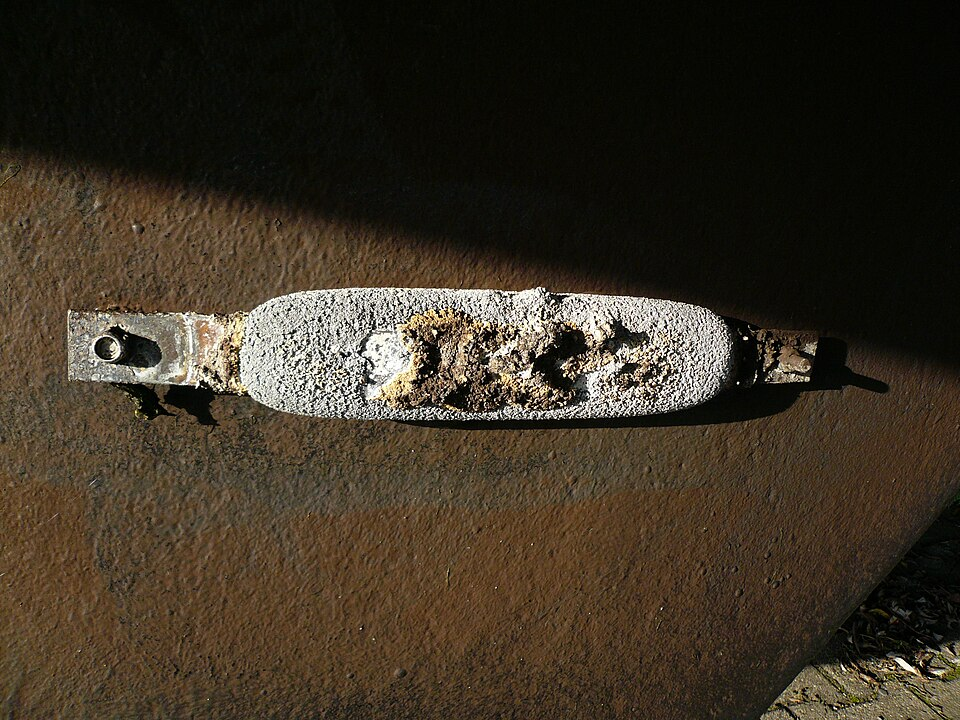
\includegraphics[width=0.5\linewidth]{images/book3/sacrificial-anode.jpg}

{\small 螺栓固定在一艘船钢制船体上的锌质牺牲阳极，经过一个季节的水中浸泡后：
锌被逐渐蚀去，周围的钢仍然完好。
（照片：Zwergelstern，CC BY-SA 3.0，维基共享资源。）}
\end{omfigure}

\begin{omfigure}
\begin{tikzpicture}[font=\small, >={Stealth}, scale=1.35]
  \begin{scope}
    \fill[black!25] (0,0) rectangle (4,0.6);
    \fill[gray!55] (0,0.6) rectangle (1.7,0.8); \fill[gray!55] (2.3,0.6) rectangle (4,0.8);
    \fill[omDef!15] (0.8,0.8) .. controls (1.3,1.3) and (2.7,1.3) .. (3.2,0.8) -- (2.3,0.8) -- (2.3,0.6) -- (1.7,0.6) -- (1.7,0.8) -- cycle;
    \node[font=\scriptsize] at (2,-0.3) {镀锌钢（锌层）};
    \node[font=\scriptsize, align=center] at (2,1.6) {锌发生腐蚀，\\ 钢受到保护};
    \draw[->, omThm] (1.4,0.85) -- (1.8,0.65);
  \end{scope}
  \begin{scope}[xshift=5.5cm]
    \fill[black!25] (0,0) rectangle (4,0.6);
    \fill[gray!25] (0,0.6) rectangle (1.7,0.8); \fill[gray!25] (2.3,0.6) rectangle (4,0.8);
    \fill[omDef!15] (0.8,0.8) .. controls (1.3,1.3) and (2.7,1.3) .. (3.2,0.8) -- (2.3,0.8) -- (2.3,0.6) -- (1.7,0.6) -- (1.7,0.8) -- cycle;
    \fill[omProp] (1.75,0.6) rectangle (2.25,0.45);
    \node[font=\scriptsize] at (2,-0.3) {镀锡钢（锡层）};
    \node[font=\scriptsize, align=center] at (2,1.6) {划痕处的钢发生腐蚀，\\ 速度快（小阳极）};
  \end{scope}
\end{tikzpicture}

{\small 穿过金属镀层的划痕示意图。锌比铁活泼，
作为阳极保护裸露的钢，无论划痕大小如何。
锡比铁惰性，在一小块钢阳极周围形成大阴极，
其腐蚀速度比裸钢更快。}
\end{omfigure}

\begin{method}[选择保护措施]\label{met:b2:corrosion:choose-protection}
\begin{enumerate}
  \item 避免形成电偶：将异种金属绝缘，或使较活泼的一方
        面积更大。
  \item 涂层：隔离性涂层（油漆、锡）仅在完好时起保护作用；
        牺牲性涂层（锌）即使被划伤也能起保护作用。
  \item 对于埋在土壤或海水中的结构，应加阴极保护：
        电流较小或水导电性强时用牺牲阳极，
        结构较长或土壤电阻大时用外加电流。
  \item 不要过度保护：电势过低时，结构表面的水
        被还原为氢气，这会使涂层脱落，并使高强度
        钢变脆。
\end{enumerate}
\end{method}

\section{练习}

\begin{exercise}[$\star$]\label{exo:b2:corrosion:1}
锌在电流密度为 \qty{2.0}{\micro A/cm^2} 时发生均匀腐蚀。
求其每年的厚度损失（$\rho = \qty{7.13}{g/cm^3}$）。
\end{exercise}

\begin{exercise}[$\star$]\label{exo:b2:corrosion:2}
用钢螺栓把铜板固定在屋顶上。哪种金属会腐蚀？
对钢板中的锌钉，提出同样的问题。
\end{exercise}

\begin{exercise}[$\star$]\label{exo:b2:corrosion:3}
两块钢板用一颗螺栓固定在一起，置于海水中。
腐蚀集中在何处？为什么？
\end{exercise}

\begin{exercise}[$\star$]\label{exo:b2:corrosion:4}
一只镀锌桶和一个镀锡罐都被划伤至钢层。哪一个
在划痕处生锈？
\end{exercise}

\begin{exercise}[$\star\star$]\label{exo:b2:corrosion:5}
在通气水中铁的埃文斯图上，说明水被搅拌时，
以及水被除去氧后，腐蚀电势与腐蚀电流
各发生什么变化。
\end{exercise}

\begin{exercise}[$\star\star$]\label{exo:b2:corrosion:6}
一块质量为 \qty{5.0}{kg} 的锌阳极，以 \qty{0.10}{A} 的电流
保护船体，电流效率为 90~\%（练习数据）。求它能
维持多长时间？
\end{exercise}

\begin{exercise}[$\star\star$]\label{exo:b2:corrosion:7}
计算锌、镁和铝阳极在 100~\% 效率下，每千克所提供的电量（以安培小时计），
并由 $\Delta_f G^\circ$ 求出它们各自电对的标准电势（
\ce{Zn^2+} $-147.06$，\ce{Mg^2+} $-454.8$，
\ce{Al^3+} $-485$ \unit{kJ/mol}）。为什么在干燥土壤中首选镁？
\end{exercise}

\begin{exercise}[$\star\star$]\label{exo:b2:corrosion:8}
一根埋地管道需要 \qty{2.0}{A} 的保护电流。惰性阳极的
接地床对土壤的电阻为 \qty{4.0}{\ohm}，电池还需
再提供 \qty{1.5}{V} 的电压（练习数据）。计算整流器的电压
和每年的电能。
\end{exercise}

\begin{exercise}[$\star\star$]\label{exo:b2:corrosion:9}
一根钢桩立于海中。解释它为何在水线稍下方
腐蚀最严重，而不在水线处本身。
\end{exercise}

\begin{exercise}[$\star\star\star$]\label{exo:b2:corrosion:10}
借助钝化曲线解释，为什么不锈钢能耐受通气水，
却可能在海水中发生点蚀，以及为什么点蚀一旦开始，
只会向深处发展而不向宽处扩展。
\end{exercise}

\begin{exercise}[$\star\star\star$]\label{exo:b2:corrosion:11}
一个铜接头拧在输送通气水的钢管上。氧的
极限电流密度在每个润湿表面上均为 \qty{5}{\micro A/cm^2}；
铜的润湿面积为 \qty{20}{cm^2}，接头附近钢的润湿面积为 \qty{2}{cm^2}
（练习数据）。估算钢的腐蚀电流，以及它在接头附近
每年的厚度损失。
\end{exercise}

\begin{exercise}[$\star\star\star$]\label{exo:b2:corrosion:12}
利用铁的 E--pH 图和水的曲线，解释为何
受保护钢结构的电势应保持在约
\qty{-0.6}{V} 以下，但在中性水中又不宜远低于 \qty{-1}{V}。
\end{exercise}

\section{问题：保护管道}

\begin{problem}[{周末问题——湿土中裸钢管的腐蚀，
牺牲金属的选择，二十年所需的镁，
以及外加电流替代方案}]
\label{pb:b2:corrosion:1}
一根长 \qty{10.0}{km}、直径 \qty{0.30}{m} 的钢管埋设于
湿土中。数据：铁 $M = \qty{55.845}{g/mol}$，$\rho = \qty{7.87}{g/cm^3}$；
镁 $M = \qty{24.305}{g/mol}$；$\Delta_f G^\circ$（\unit{kJ/mol}）：\ce{Fe^2+}
$-78.90$、\ce{Zn^2+} $-147.06$、\ce{Mg^2+} $-454.8$、\ce{Al^3+} $-485$。练习
数据：该土壤中裸钢的腐蚀电流密度为 \qty{10}{\micro
A/cm^2}；裸钢保护所用的设计电流密度为
\qty{20}{mA/m^2}；涂层使 1.0~\% 的表面裸露；镁阳极
每个 \qty{15}{kg}，效率 50~\%；外加电流所用的接地床电阻为
\qty{5.0}{\ohm}。
% ledger: aw:Fe, rho:Fe, aw:Mg, dfg:Fe2+_ao, dfg:Zn2+_ao, dfg:Mg2+_ao, dfg:Al3+_ao, const:F

\medskip
\noindent\textbf{第一部分——裸钢管。}
\begin{enumerate}
  \item 写出管道上的阳极反应和阴极反应。
  \item 为什么腐蚀电流由氧的供应所决定？
  \item 计算每平方米每年损失的铁的质量。
  \item 计算每年管壁厚度的损失量。
  \item 裸钢管损失掉 \qty{8}{mm} 管壁的一半需要多长时间？
  \item 实际管道为什么会在少数几处更早失效？
\end{enumerate}

\medskip
\noindent\textbf{第二部分——阳极金属。}
\begin{enumerate}[resume]
  \item 计算铁、锌、镁
        和铝各电对的标准电极电势。
  \item 哪些金属可以作为牺牲阳极保护铁？
  \item 为什么铝在土壤中很少使用？
  \item 为什么在高电阻率土壤中镁比锌更受青睐？
  \item 计算每安培、每年消耗的镁的质量。
\end{enumerate}

\medskip
\noindent\textbf{第三部分——设计。}
\begin{enumerate}[resume]
  \item 计算管道的外表面积。
  \item 计算涂层留下的裸露表面积。
  \item 计算保护电流。
  \item 计算二十年所需的电荷量。
  \item 计算所需镁的质量。
  \item 需要多少个阳极？
  \item 为什么阳极要沿管道分布，而不是
        集中埋在一处？
\end{enumerate}

\medskip
\noindent\textbf{第四部分——外加电流。}
\begin{enumerate}[resume]
  \item 描述外加电流方案。
  \item 由接地床电阻估算整流器的电压，
        并加上电极所需的 \qty{1.5}{V}。
  \item 计算每年消耗的电能。
  \item 若管道保护过度，会出现什么问题？
  \item 在中性水中，铁处于免蚀区的电势应低于何值，
        取亚铁离子浓度为 \qty{1e-6}{mol/L}？
  \item 给出二十年所需镁阳极的质量。
\end{enumerate}
\end{problem}
